\documentclass[10pt]{article}
\usepackage[margin=3cm]{geometry}
\usepackage{array, xcolor}
\usepackage{lipsum}
\usepackage{bibentry}
\usepackage{graphicx}
\usepackage{hyperref}

\hypersetup{%
    pdfborder = {0 0 0}
}
\title{\bfseries\Huge Franco Salvador, Marc}
\author{\href{mailto:marc.franco@symanto.com}{marc.franco@symanto.com}}
\date{}
\begin{document}
\begin{minipage}{0.65\textwidth}
\begingroup
\let\center\flushleft
\let\endcenter\endflushleft
\maketitle
\endgroup
\end{minipage}
\begin{minipage}{0.3\textwidth}
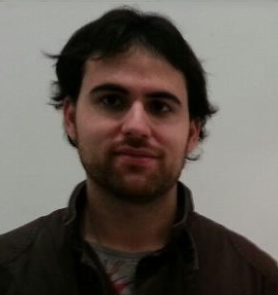
\includegraphics[scale=0.17]{img/marc}
\end{minipage}

\begin{minipage}[ht]{0.48\textwidth}
Valencia, 46184\\
Valencian Community\\
Spain
\end{minipage}
\begin{minipage}[ht]{0.48\textwidth}

\end{minipage}

\vspace{2em}


\definecolor{lightgray}{gray}{0.8}
\newcolumntype{L}{>{\raggedleft}p{0.14\textwidth}}
\newcolumntype{R}{p{0.8\textwidth}}
\newcommand\VRule{\color{lightgray}\vrule width 0.5pt}

\section*{Personal information}
\begin{tabular}{L!{\VRule}R}
Nationality&Spanish\vspace{5pt}\\
%Date of birth&06/05/1988\vspace{5pt}\\
Phone& (+34) 644 26 44 47 \vspace{5pt}\\
%LinkedIn&\href{https://www.linkedin.com/in/marfrasa/en/}{https://www.linkedin.com/in/marfrasa/en/}\\
%Google Scholar&\href{http://scholar.google.com/citations?user=tjhy5T8AAAAJ}{http://scholar.google.com/citations?user=tjhy5T8AAAAJ}\\
Websites& \href{https://www.linkedin.com/in/marfrasa/en/}{LinkedIn} $\cdot$ \href{http://scholar.google.com/citations?user=tjhy5T8AAAAJ}{Google Scholar} \\
\end{tabular}

\section*{Vocational area}
\begin{tabular}{L!{\VRule}R}
&R\&D in Multilingual Data Science, Analytics, and Mining $\cdot$ Machine and Deep Learning $\cdot$ Information Retrieval $\cdot$ Natural Language Processing \vspace{5pt}\\
\end{tabular}

\section*{Professional Experience}

\textit{References available upon request}\vspace{5pt}\\

\begin{tabular}{L!{\VRule}R}

Since Feb.~ 2021 &{\textbf{Director of Research} at \href{https://www.symanto.com/}{Symanto}, Valencia (Spain)}\\
&\scriptsize{National and international R\&D projects:}\\
&\scriptsize{\textcolor{white}{ssss}ProHaters - Proactive Profiling of Hate Speech Spreaders. 3-year R\&D project. Funded by the CDTI - Ministry of Science and Innovation, Spain (IDI-20210776).}\\
&\scriptsize{\textcolor{white}{ssss}XAI-DisInfodemics: eXplainable AI for disinformation and conspiracy detection during infodemics. 3-year R\&D project. Funded by the Ministry of Science and Innovation, Spain (PLEC2021-007681).}\\
&\scriptsize{\textcolor{white}{ssss}DETEMP - Early detection of depression symptoms in social media. 15-month R\&D project. Funded by the Valencian Institute of Business Competitiveness (IVACE), Spain (IMINOD/2021/72)}. \\&\\

Since April.~ 2021 &{\textbf{City lead} at \href{https://www.spain-ai.com/}{Valencia AI@Spain AI}, Valencia (Spain)}\\
&\\

June. 2021 -- July 2021~~~~~ &{\textbf{Collaborator - Big data \& science master} at  \href{https://www.il3.ub.edu/}{Institut de Formació Contínua IL3 - Universitat de Barcelona}, Barcelona (Spain)}\\
&\\

May 2018 -- Jan. 2021~~~ &{\textbf{Principal Research Scientist} at \href{https://www.symanto.com/}{Symanto}, Valencia (Spain)}\\&\\

Apr. 2017 -- Apr. 2018~~~ &{\textbf{Innovation Lead} at \href{https://www.symanto.com/}{Symanto}, Valencia (Spain)}\\&\\
\end{tabular}

\begin{tabular}{L!{\VRule}R}
Dec. 2016 -- ~~Apr. 2017 ~~&{\textbf{Data scientist} at \href{https://www.symanto.com/}{Symanto}, Valencia (Spain)}\\&\\
Sep. 2016 -- Nov. 2016 ~~&{\textbf{Research fellow} at \href{http://dws.informatik.uni-mannheim.de/en/home/}{Data and Web Science Group, Universit{\"a}t Mannheim}, Mannheim (Germany)}\\
&\scriptsize{Funded by DAAD (German Academic Exchange Service) in accordance with the DAAD scholarship program ``STIBET-Doktoranden''.}\\&\\

June 2016 -- ~~~Aug. 2016 ~~&{\textbf{Data scientist} at \href{https://www.symanto.com/}{Symanto}, Nuremberg (Germany)}\\&\\

July 2014 -- May 2016 ~~&{\textbf{Senior technician} at \href{http://www.prhlt.upv.es/}{Pattern Recognition and Human Language Technology (PRHLT) Research Center - Universitat Polit{\`e}cnica de Val{\`e}ncia}, Valencia (Spain)}\\
&\scriptsize{Funded by:}\\
&\scriptsize{\textcolor{white}{ssss}The Spanish Ministry of Economy and Competitiveness 3-year R\&D project (TIN2015-71147-C2-1-P) SOMEMBED - SOcial Media language 
understanding - EMBEDing contexts.}\\
&\scriptsize{\textcolor{white}{ssss}The Spanish Ministry of Economy and Competitiveness 3-year R\&D project (MEC TIN2012-38603-C02-01) DIANA-APPLICATIONS - Finding Hidden Knowledge 
in Text.}\\&\\

Apr. 2014 -- June 2014~~~~&{\textbf{Technical specialist} at \href{http://www.lsi.us.es/italica/}{It{\'a}lica Research Group - Universidad de Sevilla}, Seville (Spain)}\\
&\scriptsize{Funded by the Spanish Ministry of Economy and Competitiveness 3.5-year R\&D project (TIN2011-14726-E) \emph{Destilado de opiniones desde contenidos generados por 
usuarios.}}\\&\\
 
Apr. 2013 -- Mar. 2014 ~~&{\textbf{Research fellow} at \href{http://lcl.uniroma1.it/index.html}{Linguistic Computing Laboratory, Computer Science Department, Sapienza University of Rome}, Rome (Italy)}\\
&\scriptsize{Funded by the 5-year ERC Starting Grant No. 259234 MultiJEDI: Multilingual Joint word sEnse DIsambiguation.}\\&\\

Aug. 2012 -- Dec. 2012~~~~&{\textbf{Senior technician} at \href{http://users.dsic.upv.es/grupos/nle/}{Natural Language Engineering Lab, Department of Information Systems and Computing, Universitat Polit{\`e}cnica de Val{\`e}ncia}, Valencia (Spain)}\\
&\scriptsize{Funded by the Spanish Ministry of Education and Science 4-year R\&D project (CICYT TIN2009-13391-C04-03) TEXT-ENTERPRISE 2.0: Text comprehension techniques
applied to the needs of the Enterprise 2.0.}\\&\\
\end{tabular}

\section*{Education}
\begin{tabular}{L!{\VRule}R}
	2013--2017 &{\bf Doctor of Philosophy (PhD), Computer Science, Universitat Polit{\`e}cnica de Val{\`e}ncia, Spain}\vspace{5pt}\\
	&\textbf{Final score:} Excellent  with \textbf{cum laude} distinction\\
	&\scriptsize{PhD thesis: A Cross-domain and Cross-language Knowledge-based Representation of Text and its Meaning}\\
	&\scriptsize{Advisor: Paolo Rosso}\\
	&\\
	2011--2013&{\bf Master of Science (MSc), Artificial Intelligence, Pattern Recognition and Digital Image, Universitat Polit{\`e}cnica de Val{\`e}ncia, Spain}\vspace{5pt}\\
	&\bf Avg. score: 8.7/10\\
	&\scriptsize{MSc thesis: Cross-Language Plagiarism Detection using a Multilingual Semantic Network}\\
	&\scriptsize{Score: 10/10  -  Cum laude}\\
	&\scriptsize{Advisor: Paolo Rosso}\\
	&\\
\end{tabular}

\begin{tabular}{L!{\VRule}R}
	2006--2011& \bf Bachelor of Science (BSc), Computer Science Engineering (5-year degree), specialization in Artificial Intelligence, Universitat Polit{\`e}cnica de Val{\`e}ncia, Spain\vspace{5pt}\\
	&\bf Avg. score: 7/10\\
	&\scriptsize{BSc final project: Voice-based web surfing}\\
	&\scriptsize{Score: 10/10}\\
	&\scriptsize{Advisor: Carlos D. Mart\'inez Hinarejos}\\ 
\end{tabular}

\section*{Languages}
\begin{tabular}{L!{\VRule}R}
Spanish&Mother tongue\\
Catalan&Mother tongue\\
{\bf English}&{\bf Professional working proficiency}\\
Italian&Basic competence\\
\end{tabular}

\section*{Achievements and Awards}
\begin{tabular}{L!{\VRule}R}
  2021 & First place in several evaluation metrics at the eRisk 2021: Early risk prediction on the Internet shared task@CLEF - subtasks on "Early detection of signs of self-harm" and "Measuring the severity of the signs of depression"\vspace{5pt}\\
  2018 & PhD thesis award for the best dissertation in the field of Information Retrieval.\vspace{5pt}\\
	   &\scriptsize{Awarded by the 5th Spanish Conference in Information Retrieval (CERI 2018).}\vspace{5pt}\\
  2017 & Cum laude PhD thesis: A Cross-domain and Cross-language Knowledge-based Representation of Text and its Meaning.\vspace{5pt}\\
  2016 & First position in the \href{http://alt.qcri.org/semeval2016/task3/}{International Workshop on Se\-man\-tic Evaluation (SemEval) 2016, task 3: community question answering} - subtask B: question-question similarity.\vspace{5pt}\\
  2013 & Winner of the \href{http://www.mavir.net/premio/182-resuelto-premio-mavir-2013}{MAVIR 2013 national prize} to the best M.Sc. thesis on Language Technologies applied to Intelligent Systems of Access
  to the Multilingual and Multimedia Information.\vspace{5pt}\\
  &\scriptsize{Awarded by \href{http://www.mavir.net/}{MAVIR Consortium}. Ssponsored by C{\'o}rex and DAEDALUS.}\vspace{5pt}\\
  2013 & Cum laude MSc thesis: Cross-language Plagiarism Detection using a Multilingual Se\-man\-tic Network.\vspace{5pt}\\

  2013 & Third prize winner in the poster session of PROMISE Winter School 2013.\vspace{5pt}\\
\end{tabular}

%\section*{Tutorials}
%\begin{tabular}{L!{\VRule}R}
%Dec. 2014&Knowledge Graph-based Natural Language Processing.\\
%&\scriptsize{International Workshop on Data and Text Analytics (DATA 2014), New Delhi, India} \vspace{5pt}\\
%\end{tabular}

%\section*{Invited talks}
%\begin{tabular}{L!{\VRule}R}
%Jan. 2016&Knowledge Graph-based Cross-language and Domain Natural Language Processing.\\
%&\scriptsize{Symanto Group, Nuremberg, Germany.} \vspace{5pt}\\
%\end{tabular}
%\\
%\begin{tabular}{L!{\VRule}R}
%Feb. 2015&Semantic Relatedness using Word Representations in Vector Space.\\
%&\scriptsize{National Institute of Astrophysics, Optics and Electronics (INAOE). Puebla, Mexico.} \vspace{5pt}\\
%Jan. 2015&Learning text and word representation models.\\
%&\scriptsize{Language and Computation Center (CLiC), Universitat de Barcelona (UB), Barcelona, Spain} \vspace{5pt}\\
%Nov. 2014&Using Knowledge graphs for Natural Language Processing.\\
%&\scriptsize{International Institute of Information Technology (IIIT), Hyderabad, India} \vspace{5pt}\\
%Oct. 2014&Knowledge-based Cross-language Natural Language Processing.\\
%&\scriptsize{South Asian University (SAU). New Delhi, India.} \vspace{5pt}\\
%Nov. 2012&Graph-based Similarity Analysis: A New Approach to Cross-Language Plagiarism Detection.\\
%&\scriptsize{Computational Research Center (CIC). National Polytechnic Institute. Mexico D.F., Mexico.} \vspace{5pt}\\
%Dec. 2012&Cross-language Plagiarism Detection using a Multilingual Semantic Network.\\
%&\scriptsize{National Institute of Astrophysics, Optics and Electronics (INAOE). Puebla, Mexico.} \vspace{5pt}\\
%\end{tabular}

%\section*{Doctoral Consortium}
%\begin{tabular}{L!{\VRule}R}
%June 2014&Knowledge-based Cross-language Natural Language Processing.\\
%&\scriptsize{Presented at \emph{V Jornadas de la Red Tem{\'a}tica en Tratamiento de la Informaci{\'o}n Multiling{\"u}e y Multimodal (TIMM)}, Cazalla de la Sierra (Sevilla), Spain} \vspace{5pt}\\
%\end{tabular}

%\section*{Editorial Services to Scholarly Publications}
%Reviewer for several journals including: Artificial Intelligence; Information Sciences; Expert Systems With Applications; Journal of Intelligent and Fuzzy Systems; Language 
%Resources and Evaluation; Natural Language Engineering.

%\section*{Organising Committees}
%I have been member of the following Organising committees: Publication Co-Chair at *SEM 2015 (Joint Conference on Lexical and Computational Semantics).

%\section*{Program Committees}
%I served as member of the following program and scientific committees: ACL 2018 (Annual Meeting of the Association for Computational Linguistics), ACL 2017, IberEval@SEPLN 2018, TextGraphs@ACL 2017, KES 2017 (International Conference on Knowledge-Based and Intelligent Information \& Engineering Systems), SemEval 2016 Task 3 - Community Question Answering (International Workshop on Semantic Evaluation 2016), TIR@DEXA 2017 (International Workshop on Text-based Information Retrieval), TIR@DEXA 2016, TIR@DEXA 2015, TIR@DEXA 2014, DATA-CCIP 2015 (Special Session on DATA in International Conference on Cognitive Computing and Information Processing), SEPLN 2015 (International Workshop on Embeddings and Semantics at Spanish Conference on NLP 2015), DATA 2014 (International Workshop on Data and Text Analytics) .\\

\section*{Courses}
\begin{tabular}{L!{\VRule}R}
Oct. 2017 & \href{https://www.coursera.org/learn/cryptocurrency}{Bitcoin and Cryptocurrency Technologies}. \\
&\scriptsize{Offered by the Princeton University at Coursera}\vspace{5pt}\\
	
Feb. 2013 & \href{http://www.promise-noe.eu/events/winter-school-2013/}{PROMISE Winter School 2013 - Bridging between Information Retrieval and Databases}.\\
&\scriptsize{Bressanone, Italy.} \vspace{5pt}\\
 
Jul. 2009 & \href{http://www.uimp.es/inmersion/inmersion.html}{UIMP English Language Immersion Course - Intensive English Course with Native Teachers and Monitors}.\\
&\scriptsize{Barcelona, Spain.} \vspace{5pt}\\
\end{tabular}

\section*{Certifications}
\begin{tabular}{L!{\VRule}R}
Dec. 2021 & \href{https://raw.githubusercontent.com/neosyon/CV_latex/master/certifications/CEOE%202021%20-%20digitalizacion%20aplicada%20al%20sector%20productivo%20-%20certificado%20superacion.pdf}{Digitization applied to the productive sector}\\
&\scriptsize{Confederación Española de Organizaciones Empresariales (CEOE)} \vspace{5pt}\\
Jan. 2016 & Cambridge First Certificate in English (FCE) - B2 level of the Common European Framework of Reference for Languages (CEFR)\\
&\scriptsize{University of Cambridge} \vspace{5pt}\\
Jan. 2016 & Elemental Grade in Valencian - B1 level of the Common European Framework of Reference for Languages (CEFR)\\
&\scriptsize{Generalitat Valenciana} \vspace{5pt}\\
Dec. 2015 & Occupational safety: laboratory researcher profile (register number: 15/45480)\\
&\scriptsize{Universitat Polit{\`e}cnica de Val{\`e}ncia} \vspace{5pt}\\
\end{tabular}

\section*{Research Internships}
\begin{tabular}{L!{\VRule}R}
	2015&National Institute of Astrophysics, Optics and Electronics (INAOE), Puebla, ~~~Mexico\\
	&\scriptsize{Mentor: Dr. Manuel Montes-y-G{\'o}mez}\\          
	&\scriptsize{Funded by the  Web Information Quality Evaluation Initiative (WIQ-EI) IRSES 4-year project (grant no. 269180) within the FP 7 Marie Curie People Framework.}\\
	&\scriptsize{Date: Feb. - Mar. 2015}\vspace{5pt}\\
	2014&International Institute of Information Technology (IIIT), Hyderabad, India\\
	&\scriptsize{*During this internship I have been also research intern at Veooz - URL: \url{www.veooz.com} }\\
	&\scriptsize{Mentor: Prof. Dr. Vasudeva Varma}\\          
	&\scriptsize{Funded by the  Web Information Quality Evaluation Initiative (WIQ-EI) IRSES 4-year project (grant no. 269180) within the FP 7 Marie Curie People Framework.}\\
	&\scriptsize{Date: Oct - Dec. 2014}\vspace{5pt}\\
	2012&Computational Research Center (CIC), Mexico D.F., Mexico \& National Institute of Astrophysics, Optics and Electronics (INAOE), Puebla, Mexico\\
	&\scriptsize{Mentor: Prof. Dr. Grigori Sidorov \& Dr. Manuel Montes-y-G{\'o}mez}\\          
	&\scriptsize{Funded by the  Web Information Quality Evaluation Initiative (WIQ-EI) IRSES 4-year project (grant no. 269180) within the FP 7 Marie Curie People Framework.}\\
	&\scriptsize{Date: Nov - Dec. 2012}\vspace{5pt}\\
\end{tabular}

\section*{Competences}
\begin{tabular}{L!{\VRule}R}
Artificial Intelligence\\&Deep learning, machine learning, data mining, natural language processing, information retrieval, machine translation\\
Data Mining \& Machine Learning\\&TensorFlow, Keras, PyTorch, scikit-learn, huggingface-transformers, Weka\\
Programming Languages\\&Python, Java, C, C++, Bash\\
Software Development\\&Kanban, Scrum, Eclipse, Maven, Visual Studio, Visual Studio Code, Git\\
Containers \& Orchestration\\ & Docker, Kubernetes\\
Big Data, DB\\& Spark, SQL, PostgreSQL, Oracle\\
%Social Competences\\&Teamwork capacity, capacity of adaptation to multicultural environments\\
%Organizational Competences\\&Good communication, planning and organizational skills, availability to travel\\
\end{tabular}

\section*{Publications}
\begin{tabular}{L!{\VRule}R}
	2021 & C. Cohrdes, S. Yenikent, J. Wu, B. Ghanem, M. Franco-Salvador, and F. Vogelgesang. \textbf{Indications of Depressive Symptoms During the COVID-19 Pandemic in Germany: Comparison of National Survey and Twitter Data.}
	In \emph{JMIR Ment Health} 2021;8(6):e27140, DOI: \href{https://doi.org/10.2196/27140}{10.2196/27140} \textbf{(Impact Factor: 4.39)} \vspace{5pt}\\
	2021 & A. Basile, G. P{\'e}rez-Torr{\'o}, and M. Franco-Salvador. \textbf{Probabilistic Ensembles of Zero- and Few-Shot Learning Models for Emotion Classification.}
	In \emph{Proc. of the International Conference on Recent Advances in Natural Language Processing (RANLP 2021)}, Bulgaria, September 1-4, pp. 128--137. \vspace{5pt}\\
	2021 & A. Basile, M. Chinea-Rios, A.S. Uban, T. Muller, L. Rossler, S. Yenikent, B. Chulv{\'i}, P. Rosso, and M. Franco-Salvador. \textbf{UPV-Symanto at eRisk 2021: Mental Health Author Profiling for Early Risk Prediction on the Internet.}
	In \emph{CLEF 2021 Labs and Workshops, Notebook Papers.} CEUR-WS.org, \href{http://ceur-ws.org/Vol-2936/paper-75.pdf}{http://ceur-ws.org/Vol-2936/paper-75.pdf}. \vspace{5pt}\\
	2021 & S. Stajner, S. Yenikent, B. Ghanem, and M. Franco-Salvador. \textbf{What Motivates You? Benchmarking Automatic Detection of Basic Needs From Short Posts.}
	In \emph{Proc. of the Joint Conference of the 59th Annual Meeting of the Association for Computational Linguistics and the 11th International Joint Conference on Natural Language Processing (ACL-IJCNLP 2021)}, August 1th through August 6th, 2021, pp.  803-–81. \textbf{(CORE A)}\vspace{5pt}\\
	2021 & S. Stajner, S. Yenikent, and M. Franco-Salvador. \textbf{Five Psycholinguistic Characteristics for Better Interaction with Users.}
	In \emph{Proceedings of the 8th IEEE International Conference on Behavioural and Social Computing (BESC)}, November 1, 2021.\vspace{5pt}\\	
\end{tabular}
\section*{}
\begin{tabular}{L!{\VRule}R}
	2020 & M. Chinea-Rios, M. Franco-Salvador, and Y. Benajiba. \textbf{Aspect On: an Interactive Solution for Post-Editing the Aspect Extraction based on Online Learning.}
	In \emph{Proceedings of The 12th Language Resources and Evaluation Conference (LREC 2020)}, Marseille, France, May 13-16, pp. 4974--4981. 	\textbf{(CORE C)}\vspace{5pt}\\	
	2019 & A. Basile, M. Franco-Salvador, N. Pawar, S. \v{S}tajner, M. Chinea Rios, and Y. Benajiba. \textbf{SymantoResearch at SemEval-2019 Task 3: Combined Neural Models for Emotion Classification in Human-Chatbot Conversations.}
	In \emph{Proceedings of the 13th International Workshop on Semantic Evaluation (SemEval-2019)}, Minneapolis, USA, June 6-7.\vspace{5pt}\\	
	2018 & M. Franco-Salvador, and L. A. Leiva. \textbf{Multilingual phrase sampling for text entry evaluations.}
	In \emph{International Journal of Human-Computer Studies}, vol. 113, pp. 15-31. \href{https://doi.org/10.1016/j.ijhcs.2018.01.006}{DOI: 10.1016/j.ijhcs.2018.01.006} \textbf{(Impact Factor: 2.13)} \vspace{5pt}\\	
	2018& R. M. Gim{\'e}nez-P{\'e}rez, M. Franco-Salvador, and P. Rosso. \textbf{String Kernels for Polarity Classification: A Study across Different Languages.}
	In \emph{Proc. of the 23rd International Conference on Natural Language \& Information Systems (NLDB 2018)}, Paris, France, 13-15 June, pp. 489--493. \textbf{(CORE C)}\vspace{5pt}\\
	2018&M. A. {\'A}lvarez Carmona,  M. Franco-Salvador, M. Montes-Y-G{\'o}mez, P. Rosso, L. Villase{\~n}or-Pineda, and E. Villatoro Tello. \textbf{Semantically-informed Distance and Similarity Measures for Paraphrase Plagiarism Identification.}
	In \emph{Journal of Intelligent and Fuzzy Systems, Special Issue 4th Int. Symposium on Language \& Knowledge Engineering}, vol. 34, pp. 2983--2990. \href{https://doi.org/10.3233/JIFS-169483}{DOI: 10.3233/JIFS-169483} \textbf{(Impact Factor: 1.26)} \vspace{5pt}\\	
	2018 & S. \v{S}tajner, M. Franco-Salvador, P. Rosso, and S. P. Ponzetto. \textbf{CATS: A Tool for Customised Alignment of Text Simplification Corpora.} In \emph{Proc. 11th Int. Conf. on Language Resources and Evaluation (LREC 2018)}, Miyazaki, Japan, May 7-12. \textbf{(CORE C)} \vspace{5pt}\\
	2017 & G. Glava{\v s}, M. Franco-Salvador, S. P. Ponzetto, and P. Rosso. \textbf{A Resource-light Method for Cross-lingual Semantic Textual Similarity.}
	In \emph{Knowledge-Based Systems}, vol. 143, pp. 1-9. \href{https://doi.org/10.1016/j.knosys.2017.11.041}{DOI: 10.1016/j.knosys.2017.11.041} \textbf{(Impact Factor: 4.53)} \vspace{5pt}\\	
	2017& S. \v{S}tajner, M. Franco-Salvador, S. P. Ponzetto, P. Rosso, and H. Stuckenschmidt. \textbf{Sentence Alignment Methods for Improving Text Simplification Systems.}
	In \emph{Proc. of the 55th Annual Meeting of the Association for Computational Linguistics (ACL 2017)},  Vancouver, Canada, July 30th through August 4th, 2017, pp. 97--102. \textbf{(CORE A)}\vspace{5pt}\\
	2017& M. Franco-Salvador. \textbf{A Cross-domain and Cross-language Knowledge-based Representation of Text and its Meaning.}
	In \emph{PhD Thesis, Universitat Polit{\`e}cnica de Val{\`e}ncia.} \href{http://hdl.handle.net/10251/84285}{http://hdl.handle.net/10251/84285}\vspace{5pt}\\
	2017& M. Franco-Salvador, N. Plotnikova, N. Pawar, and Y. Benajiba. \textbf{Subword-based Deep Averaging Networks for Author Profiling in Social Media - Notebook for PAN at CLEF 2017.}
	In \emph{CLEF 2017 Labs and Workshops, Notebook Papers.} CEUR-WS.org, \href{http://ceur-ws.org/Vol-1866/}{http://ceur-ws.org/Vol-1866/} \vspace{5pt}\\
\end{tabular}
\section*{}
\begin{tabular}{L!{\VRule}R}	
	2017&M. Franco-Salvador, Greg Kondrak, and P. Rosso. \textbf{Bridging the Native Language and Language Variety Identification Tasks.}
	In \emph{Proc. of the 21st International Conference on Knowledge-Based and Intelligent Information \& Engineering Systems (KES 2017)}, Marseille, France, 6-8 September, 2017, pp. 1554--1561. \href{https://doi.org/10.1016/j.procs.2017.08.068}{DOI: 10.1016/j.procs.2017.08.06} \textbf{(CORE B)}\vspace{5pt}\\
	2017&R. M. Gim{\'e}nez-P{\'e}rez, M. Franco-Salvador, and P. Rosso. \textbf{Single and Cross-domain Polarity Classification using String Kernels.}
	In \emph{Proc. of the 15th Conference of the European Chapter of the Association for Computational Linguistics (EACL 2017)}, Valencia, Spain, 3-7 April, 2017, pp. 558-563. \textbf{(CORE A)}\vspace{5pt}\\
	2016&M. Franco-Salvador, P. Gupta, P. Rosso, and R. E. Banchs. \textbf{Cross-language Plagiarism Detection Over Continuous-space- and Knowledge Graph-based Representations of Language.}
	In \emph{Knowledge-Based Systems}, vol. 111, pp. 87--99. \href{http://dx.doi.org/10.1016/j.knosys.2016.08.004}{DOI: 10.1016/j.knosys.2016.08.004} \textbf{(Impact Factor: 4.53)} \vspace{5pt}\\
	2016&M. Franco-Salvador, P. Rosso, and M. Montes-y-G{\'o}mez. \textbf{A Systematic Study of Knowledge Graph Analysis for Cross-language Plagiarism Detection.}
	In \emph{Information Processing \& Management}, vol. 52(4), pp. 550--570. \href{http://dx.doi.org/10.1016/j.ipm.2015.12.004}{DOI: 10.1016/j.ipm.2015.12.004} \textbf{(Impact Factor: 2.39)} \vspace{5pt}\\
	2016 &M. Franco-Salvador, S. Kar, T. Solorio, and P. Rosso. \textbf{UH-PRHLT at SemEval-2016 Task 3: Combining Lexical and Semantic-based Features for Community Question Answering.} In \emph{Proc. of the 10th International Workshop on Semantic Evaluation, SemEval '16}, San Diego, California. Association for Computational Linguistics. \vspace{5pt}\\
	2016 &F. Rangel, M. Franco-Salvador, and P. Rosso. \textbf{A Low Dimensionality Representation for Language Variety Identification.} In \emph{Proc.  of  the  17th  International Conference on Intelligent Text Processing and Computational Linguistics (CICLing 2016)}, Springer, Cham, 2016. pp. 156-169. \vspace{5pt}\\
	2015&M. Franco-Salvador, F. L. Cruz, J. A. Troyano, and P. Rosso. \textbf{Cross-domain Polarity Classification using a Knowledge-enhanced Meta-classifier.}	
	In \emph{Knowledge-Based Systems}, vol. 86, pp. 46--56. \href{http://dx.doi.org/10.1016/j.knosys.2015.05.020}{DOI: 10.1016/j.knosys.2015.05.020} \textbf{(Impact Factor: 4.53)} \vspace{5pt}\\
	2015&M. Franco-Salvador, F. Rangel, P. Rosso, M. Taul{\'e}, and A. Mart{\'i}. \textbf{Language Variety Identification using Distributed Representations of Words and Documents.}
	In \emph{6th International Conference of CLEF on Experimental IR meets Multilinguality, Multimodality, and Interaction (CLEF 2015)}, Springer-Verlag, LNCS(9283), pp. 28--40. \vspace{5pt}\\
	2015&M. Franco-Salvador, I. Bensalem, E. Flores, P. Gupta, and P. Rosso. \textbf{PAN 2015 Shared Task on Plagiarism Detection: Evaluation of Corpora for Text Alignment.}
	In \emph{CLEF 2015 Labs and Workshops, Notebook Papers.} CEUR-WS.org, \href{http://ceur-ws.org/Vol-1391/}{http://ceur-ws.org/Vol-1391/} \vspace{5pt}\\
	2015&M. Franco-Salvador, P. Rosso, and F. Rangel. \textbf{Distributed Representations of Words and Documents for Discriminating Similar Languages.}
	In \emph{Proc. of the RANLP Joint Workshop on Language Technology for Closely Related Languages, Varieties and Dialects (LT4VarDial)}. \vspace{5pt}\\
\end{tabular}
\section*{}
\begin{tabular}{L!{\VRule}R}
	2014&M. Franco-Salvador, P. Rosso, and R. Navigli. \textbf{A Knowledge-based Representation for Cross-Language Document Retrieval and Categorization.}
	In \emph{Proc. of the 14th Conference of the European Chapter of the Association for Computational Linguistics (EACL 2014)}, Gothenburg, Sweden, 26-30 April, 2014, pp. 414--423. \textbf{(CORE A)} \vspace{5pt}\\
	2014&M. Franco-Salvador, P. Gupta and P. Rosso. \textbf{Knowledge Graphs as Context Models: Improving the Detection of Cross-Language Plagiarism with Paraphrasing.}
	In \emph{Revised Papers PROMISE Winter School 2013}, Springer-Verlag, LNCS(8173), pp. 227--236.\vspace{5pt}\\
	2013&M. Franco-Salvador, P. Gupta and P. Rosso. \textbf{Graph-Based Similarity Analysis: A New Approach to Cross-Language Plagiarism Detection.}
	In \emph{Sociedad Espa{\~n}ola de Procesamiento del Languaje Natural (SEPLN)}, num. 50, pp. 21--28. \vspace{5pt}\\
	2013&M. Franco-Salvador, P. Gupta and P. Rosso. \textbf{Cross-Language Plagiarism Detection using a Multilingual Semantic Network.}
	In \emph{Proc. of the 35th European Conference on Information Retrieval (ECIR 2013)}, Moscow, Russia, 24-27 March, 2013, Springer-Verlag, LNCS(7814), pp. 710--713. \textbf{(CORE B)}\vspace{5pt}\\
	2012&M. Franco-Salvador, P. Gupta and P. Rosso. \textbf{Cross-language Plagiarism Detection Using BabelNet's Statistical Dictionary.}
	In \emph{Computaci{\'o}n y Sistemas, Revista Iberoamericana de Computaci{\'o}n}, ISSN 1405-5546, vol. 16, num. 4, pp. 383--390.\vspace{5pt}\\
\end{tabular}

\end{document}
\grid
